\chapter{Theoretical Background}\label{sec:basics}

This chapter presents the theoretical background of this thesis. We will explain the foundations of quantitative information flow control and the different measures that are used to quantify information leakage. Furthermore, we will outline important aspects of (approximate) model counting, as well as basic principles used in static (Q)IFC analyses \emph{Nildumu} and \emph{JOANA}, as both are used in our hybrid QIFC tool.

\section{Quantitative Information Flow Control}

Information flow control aims to guarantee the confidentiality of the secret input data of a program, by examining the flow of information through the program to public output channels, where the information would become accessible to an attacker.

There are different ways in which such information leakage might happen: Explicit information flows are a consequence of data dependencies. They occur for example when a secret values itself is written to a public channel or the information is copied to a variable that is later leaked to a public channel. An example of a program is shown in figure \ref{fig:exEx}. Implicit information flows are caused by control dependencies. Leaks through implicit flows happen when secret values affect the program's output by influencing the execution path. Figure \ref{fig:ifEx} shows a program that contains an implicit flow. The program never assigns a secret value to an output variable. However, through the condition of the if-statement, the secret still has an influence on the output value. 
Additional to explicit and implicit flows, an attacker could gain information trough covert channels by observing a program's usage of different resources, such as time or memory \cite{smith07}.

The aim of qualitative information flow control is to prove the absence of explicit and implicit information flows, a property called \emph{non-interference}. For real world applications, leaking a certain amount of information is often required to build useful programs. In this case, the non-interference property is too strict. Instead, we wish to limit the amount of information that is leaked. Quantitative information flow control provides tools to measure how much information can be learned by an attacker about a program's secret inputs \cite{smith09}.

The central question of QIFC is: Given a program \p that accepts some input \In and produces some output \Out, how much information can an adversary \A learn about \In, if he knows the program \p and observes \Out?

We will use the following assumptions for \p and \A:

\paragraph{Input program}\label{p:input} We assume \p to be a sequential, deterministic program, that receives an input $\mIn$ and produces an output $\mOut$. Both the input and output can be tuples that consist of multiple values. The concrete input and output values of a single execution are called $h$ and $l$. The input $h$ is an element of the set of all possible inputs for a program $mIn$. We assume that all program executions terminate.

Because the programs we consider are deterministic, each program $p$ and input value $h$ induces a mapping $\llbracket p \rrbracket_h: \{\mOut\} \longrightarrow \mathcal{L}$, where $\mathcal{L}$ is the set of all possible outputs of the program. The set $\mathcal{L}$ is determined by $p$ and $\mIn$ via the equation $\mathcal{L} := \{\llbracket p \rrbracket_h(\mOut) \: | \: h \in \mIn \}$

For a  more detailed description of the input language we used, we refer to \ref{sec:inputLang}.

\paragraph{Security Lattice} Input and output variables are associated with an element of a security lattice, describing its confidentiality level. We use a lattice with two elements: $\hat{l}$ for public values and $\hat{h}$ for secret values. If not otherwise specified, we consider all inputs to be high and all outputs to be low.
% Schneider -- nur high und low

\paragraph{Attacker Model} We consider an adversary \A that knows the source code of the program \p and observes all outputs with a low security level after the execution finished. The input value for an execution are chosen based on an underlying probability distribution, which is also known to the adversary.

We assume that the attacker is not able to extract any information through covert channels. The goal of the attacker is to guess the secret input of the program, using the information he can extract through observing the program's output.

%% standard def von min etropy aus smith paper funzt nicht für public inputs
%% new notion (min-entropy ???)
%% handbuch for quantitative information flow

% many leakage measures use average over all possible executions (min entropy, Shannon entropy)
% leakage can differ greatly between different executions --> example algorithm 1
% want to measure amount of information attacker has about the input after a single program execution

\begin{figure}
    \centering
    \begin{minipage}{.7\linewidth}
        \begin{algorithm}[H]
            \hspace*{\algorithmicindent} \textbf{Input} \In: int \\
            \hspace*{\algorithmicindent} \textbf{Output} \Out: int
            \hspace*{1em}
            \begin{algorithmic}[1]
                \State $\mOut: int \leftarrow \mIn \: \% \: 10$
            \end{algorithmic} 
        \end{algorithm}
\end{minipage}
\caption{Example for information leakage through explicit flows, caused by a data dependency in line 1}
\label{fig:exEx}
\end{figure}

\begin{figure}
    \centering
    \begin{minipage}{.7\linewidth}
        \begin{algorithm}[H]
            \hspace*{\algorithmicindent} \textbf{Input} \In: int \\
            \hspace*{\algorithmicindent} \textbf{Output} \Out: int
            \hspace*{1em}
            \begin{algorithmic}[1]
                \State $\mOut: int \leftarrow 0$
                \If{ $\mIn == 42$}
                \State $\mOut \leftarrow 1$
                \EndIf
            \end{algorithmic} 
        \end{algorithm}
\end{minipage}
\caption{Example for information leakage through implicit flows, caused by a control dependency from line 2 to line 3}
\label{fig:ifEx}
\end{figure}

\paragraph{Information Flow Measures}\label{ch:measures}

Smith \cite{smith09} characterizes information leakage with the following informal equation:
\begin{center}
    \begin{equation}
        \text{Initial uncertainty} = \text{information leaked} + \text{remaining uncertainty}
    \end{equation}\label{eq:measure}
\end{center}
In our scenario, the unknown value \In is the initial uncertainty, measured by some entropy measure. The remaining uncertainty is the entropy of \In after observing \Out.

\paragraph*{Measuring Leakage with Vulnerability}
A widely used measure for information leakage is \emph{min-entropy}, which is based on vulnerability. Following the definitions from \cite{smith09}, the vulnerability of a value $X$ describes \enquote{the worst case probability that an adversary could guess the value of $X$ in one try.}

\begin{definition}[Vulnerability and Min-Entropy]\label{def:vul}
    Let $X$ be a random variables and $\mathcal{X}$ the set of possible values for $X$. The \emph{vulnerability} $V(X)$ is defined as
    \begin{center}
        $V(X) := \max\limits_{x \in \mathcal{X}} P[X = x]$
    \end{center}
    The min-entropy of $X$ is given by
    \begin{center}
        $H_\infty (X) := \log_2 \frac{1}{V(X)}$
    \end{center}
\end{definition}

\begin{definition}[Conditional Entropy]
    Given two random variables $X$ and $Y$ that are jointly distributed, the conditional entropy $H(X \: | \: Y)$ describes the uncertainty about $X$ given $Y$. $H(X \: | \: Y)$ is defined as 
    \begin{center}
        $H(X \: | \: Y) := \sum\limits_{y \in \mathcal{Y}} P[Y = y] H(X \: | \: Y = y)$
    \end{center}
    where
    \begin{center}
        \begin{equation}\label{eq:dynEntropy}
        H(X | Y = y) := \sum\limits_{x \in \mathcal{X}} P[X = x | Y = y] \log \frac{1}{P[X = x | Y = y]}
    \end{equation}
    \end{center}
    
\end{definition}

Using these definitions, Smith \cite{smith09} proposes the following definitions for the leakage equation in \ref{eq:measure}:

The initial uncertainty is given by the min-entropy of the input value $H_\infty(\mIn)$ and the remaining uncertainty is given by the conditional min-entropy $H_\infty(\mIn \: | \: \mOut)$ of $\mIn$ after having observed $\mOut$ as the output.

Thus the information leaked by a program is $H_\infty(\mIn) - H_\infty(\mIn \: | \: \mOut)$. This quantity can be determined easily with the following definition and theorem:

\begin{definition}[Channel Capacity]
    Given a program $p$, the channel capacity of $p$ is the logarithm of the number of distinct outputs than can be produced by $p$.
    \begin{center}
        $cc(p) := \log_2 |\mathcal{L}|$
    \end{center}
    For deterministic programs, the channel capacity is the maximum entropy of $\mOut$ over all distributions of $\mathcal{H}$ \cite{smith09}.
\end{definition}

\begin{theorem}[Measuring Min-entropy through Channel Capacity]
    For deterministic programs $p$, with $\mathcal{H}$ being uniformly distributed, the information leaked is equal to the channel capacity of $p$.
\end{theorem}

\paragraph{Measuring Leakage for Individual Program Executions}
While the vulnerability-based approach is appropriate to assess the risk of inadvertent information leakage for the program as a whole, it fails to give realistic measures in the dynamic case. If we consider the output of a single program run, the information an attacker may obtain from the output can be significantly greater than what the channel capacity of the program tells us  \cite{bielova16}.

We demonstrate this using the example program from \ref{fig:ifEx}. The possible outputs of the program are \texttt{0} and \texttt{1}, so the leakage, measured in bits, using the channel capacity formula is $\log_2 2 = 1$ Assuming integers are 64 bit wide, leaking a single bit seems acceptable in most cases.

Now, let's assume we run the program with the input $h := 42$. The output of the program will be $1$. An attacker that observes this output and has access to the program text will now know that the secret input was $42$. Instead of one single bit, the attacker has gained knowledge about all 64 bit of the secret input. For every other input, the attacker can only conclude that $\mIn \neq 42$. That leaves $2^{64} - 1$ possible inputs that are indistinguishable for the attacker. 

This example shows that relying on min-entropy and channel capacity as a measure of information leakage can be dangerous if we care about the confidentiality of the secret inputs in every run of the program. Therefore, we now introduce measures, that are more suited for the dynamic case.

We define an equivalence relation called the \emph{indistinguishability relation} as shown in definition \ref{def:ir}, where two inputs are related iff they produce the same program output. The equivalence class of this relation are pre-images of the possible program outputs (see definition \ref{def:is}). When the adversary observes the value $l$, he knows that the secret input must be an element of $\mathcal{H}_l$. Thus, the bigger the size of $\mathcal{H}_l$, the less likely the adversary is, to guess the secret input in a single try \cite{backes09, smith09, alvim19}. 

\begin{definition}[Indistinguishability Relation]\label{def:ir}
        For each program $p$, we define the \emph{indistinguishability relation} $\thicksim$ over $\mathcal{H}$ as:
        \begin{center}
            $\forall h, h' \in \mathcal{H}: h \thicksim  h' \iff \llbracket p \rrbracket_h(\mOut) = \llbracket p \rrbracket_{h'}(\mOut)$
        \end{center}
\end{definition}

\begin{definition}[Indistinguishability Set]\label{def:is}
    The indistinguishability set of a public output $l \in \mathcal{L}$ of a program $p$ is given as:
    \begin{center}
        $\mathcal{H}_l :=\{ h \in \mathcal{H} \: | \: \llbracket p \rrbracket_h(\mOut) = l \}$
    \end{center}
\end{definition}

Consequently, in the dynamic case the probability of an attacker guessing the secret in a single try depends on the size of the indistinguishability set for the output for the specific execution that is analyzed.

To reflect this notion in the leakage measure of our analysis, we redefine the \emph{remaining uncertainty} in equation \ref{eq:measure} as the conditional entropy of $\mIn$, given the outcome $\mOut = l$. The formula of this quantity is given in equation \ref{eq:dynEntropy}.

As mentioned above, the possible values for $\mIn$ are restricted to the elements of $\mathcal{H}_l$, so the probability $P[H = h | L = l] = 0$ for all $h \in \mathcal{H} \setminus \mathcal{H}_l$. Assuming a uniform distribution for the secret input values, we obtain the following leakage measure:

\begin{align*}
    H(\mathtt{H} | \mathtt{L} = l) &:= \sum\limits_{h \in \mathcal{H}} P[\mIn = h | \mOut = l] \log_2 \frac{1}{P[\mIn = h | \mOut = l]} \\[1em]
    &= \sum\limits_{h \in \mathcal{H}_l} \frac{1}{|\mathcal{H}_l|} \log_2 |\mathcal{H}_l| \\[1em]
    &= \log_2 |\mathcal{H}_l|
\end{align*}

\begin{theorem}[Dynamic leakage]
    Assuming a uniform distribution of the inputs, the dynamic leakage of a single program run of a program $p$ with a resulting output $l$ is given by 
    \begin{align*}
        L_{dyn}(p, l) &:= H_\infty(\mIn) - H(\mIn | \mOut = l) \\[1em]
        &= \log_2 |\mathcal{H}| - \log_2 |\mathcal{H}_l|
    \end{align*}
\end{theorem}

The table in figure \ref{tab:comp} compares the two leakage measures defined in this section.

The relationship between dynamic leakage and min-entropy is shown in equation \ref{eq:ev}: The channel capacity of a program is corresponds to the expected value of the dynamic leakage. The proof for the equation is given in the appendix \ref{ch:evProof}.

\begin{center}
    \begin{equation}\label{eq:ev}
        cc(p) = \mathbb{E}(L_{dyn}(p, l))
    \end{equation}
\end{center}

\td{finish -- clean up some of the definitions + theorems -- citations}

\begin{figure}
    \centering
    \begin{tabular}{ |c|c|c| } 
        \hline
        observed output & channel capacity & dynamic leakage \\
        \hline
        $\mOut = 1$ & $2$ & $64$ \\ 
        $\mOut = 0$ & $2$ & $7.8 * 10^{-20}$ \\ 
        \hline
    \end{tabular}
    \caption{Comparison of the two leakage measures for example \ref{fig:exEx}. The quantities are measured in bit.}
    \label{tab:comp}
\end{figure}

\section{Program Representation}

\paragraph{Control Flow Graph}
A control flow graph (CFG) is a program representation that highlights the control flows and possible execution paths in the program \cite{allen70}. CFGs are widely used in compiler optimizations and static program analyses. The nodes of a CFG are a function's basic blocks, plus two special blocks \texttt{start} and \texttt{end}, that mark the single entry- and exit point of the function. An edge is inserted for every possible jump from one block to another. An example graph for the program from figure \ref{fig:ifEx} can be seen in \ref{fig:cfg}.

We use $\mbb_p$ for the set of all basic blocks of a program \p and $b_1, b_2, ...$ for the blocks themselves. With exception of the \texttt{start}- and \texttt{end}-block, every block in the CFG has at minimum one predecessor and one successor.

\paragraph{Static Single Assignment}
Static single assignment (SSA) is a representation of the program, where every variable is assigned exactly once. If in the original program, a variable is written to more than once, a copy of the variable is created, that replaces the original one from that point in the program \cite{rosen88}. 

 To decide which copy of a variable reaches a statement that uses the value of that variable, $\phi$-functions are used. $\phi$-functions are placed at points in the program at which multiple control flow paths merge. In a CFG these point are basic blocks that have more than one predecessor. For each control flow path, the variable copy used on that path is given as an argument to the $\phi$-function. During execution, the $\phi$-function evaluates to the argument that belongs to the control flow path, that was executed. The CFG in figure \ref{fig:cfg} contains a $\phi$-function in block $b_3$. The value $\mOut$ defined in $b_3$ is assigned the value $\mOut_1$, if block $b_2$ is executed, otherwise $\mOut_0$ will be assigned to $\mOut$.

All data structures we use to represent the input program, are built using the SSA-form of the program.

\paragraph{Program Dependence Graph}
A program dependence graph (PDG) is an intermediate representation of a program that makes the programs data and control dependencies explicit. Its nodes are the programs operations and expressions and the edges represent the dependencies that exist between those \cite{ferrante84}. The Program Dependence Graph of \ref{fig:ifEx} is shown in figure \ref{fig:pdg}.

A data dependency edge from node $x$ to node $y$ exists, if the operation of the node $y$ depends on a value that is defined in the node $x$.

A control dependency edge from node $x$ to node $y$ exists, if the outcome of $x$ has influence on whether node $y$ will be executed.

Thus, a path $x \stackrel{*}{\rightsquigarrow } y$ between two nodes exists, if information can flow in the program from location $x$ to location $y$. Consequently, if there is no path, no information can flow between the two statements. This property makes PDGs a popular data structure for information flow analysis \cite{horwitz88,giffhorn12}.

\begin{figure}
    \begin{subfigure}[t]{.45\textwidth}
        \centering
            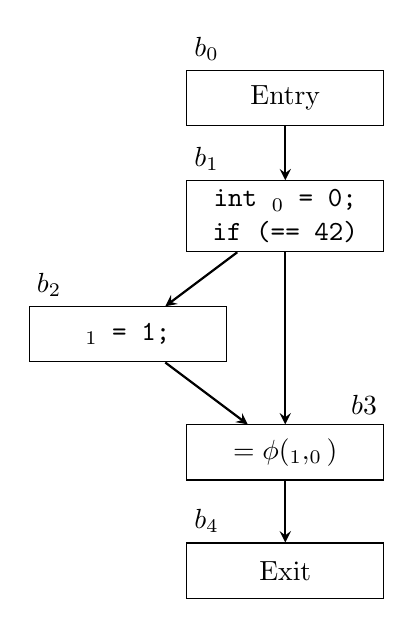
\begin{tikzpicture}
                \tikzstyle{node} = [rectangle, minimum width=2.5cm, minimum height=.7cm, text centered, draw=black, node distance=1.5cm]
                \tikzstyle{arrow} = [thick,->,>=stealth]
                
                \node (entry) [node, label={[xshift=-1cm]$b_0$}] {Entry};
                \node (b1) [node, below of=entry, align=center, label={[xshift=-1cm]$b_1$}] {\texttt{int $\mOut_0$ = 0;} \\ \texttt{if (\In == 42)}};
                \node (b2) [node, below of=b1, xshift=-2cm, label={[xshift=-1cm]$b_2$}] {\texttt{$\mOut_1$ = 1;}};
                \node (b3) [node, below of=b2, xshift=+2cm, align = center, label={[xshift=1cm]$b3$}] {$\mOut = \phi(\mOut_1, \mOut_0)$};
                \node (exit) [node, below of=b3, label={[xshift=-1cm]$b_4$}] {Exit};

                \draw [arrow] (entry) -- (b1);
                \draw [arrow] (b1) -- (b2);
                \draw [arrow] (b1) -- (b3);
                \draw [arrow] (b2) -- (b3);
                \draw [arrow] (b3) -- (exit);
            \end{tikzpicture}
        \caption{Control Flow Graph}
        \label{fig:cfg}
    \end{subfigure}\hfill
    \begin{subfigure}[t]{.45\textwidth}
        \centering
        \begin{tikzpicture}
            \tikzstyle{node} = [ellipse, minimum width=2.5cm, minimum height=.7cm, text centered, draw=black, node distance=2cm]
            \tikzstyle{arrow} = [thick,->,>=stealth]
            
            \node (b1) [node] {\texttt{int $\mOut_0$ = 0;}};
            \node (b2) [node, below left of=b1] {\texttt{\In == 42}};
            \node (b3) [node, below of=b2] {\texttt{$\mOut_1$ = 1;}};
            \node (b33) [node, below right of=b3] {$\mOut = \phi(\mOut_1, \mOut_0)$};

            \draw [arrow] (b1) -- (b33);
            \draw [arrow, blue] (b2) -- (b3);
            \draw [arrow] (b3) -- (b33);
        \end{tikzpicture}
        \caption{Program Dependence Graph\\The black edges are data dependencies, while blue edges show control dependencies}
        \label{fig:pdg}
    \end{subfigure}
    \caption{Different graph representations for the program in \ref{fig:ifEx}}
\end{figure}


\section{Program Slicing}

\com{put in new section: static techniques? could also include some stuff about what nildumu does}

Slicing is a technique used to find those sections of a program, that are influenced by (forward slice) or influence (backward slice) a given location in the program \cite{weiser81}.
This location is called the \emph{slicing criterion} and is a tuple $\langle s, v \rangle$ of a program statement $s$ and a variable $v$.
The \emph{backward slice} with respect to the criterion $\langle s, v \rangle$ contains all statements that influence the value of $v$ at point $s$ in the program. 
A \emph{forward slice} with respect to the criterion $\langle s, v \rangle$ contains all statements that are influenced by the value of $v$ assigned at point $s$ in the program.

Computing a program slice can be efficiently done using the PDG of the given program. Since all dependencies are explicitly represented as edges, the computation of a program slice is reduced to a reachability problem \cite{ottenstein84}: 

The backward slice for a node $v$ is given as the set of all nodes $v'$, for which a path $v' \stackrel{*}{\rightsquigarrow} v$ exists. The forward slice of node $v$ is given as the set of all nodes $v'$, for which a path $v \stackrel{*}{\rightsquigarrow} v'$ exists.

Horwitz \cite{horwitz88sdg} noted that interprocedural slices could be computed similarly using system dependence graphs.

Tools like JOANA use slicing techniques on system dependence graphs to analyse the information flow in programs and give non-interference guarantees where possible \cite{hammer09}.

\begin{figure}
    \centering
    \begin{minipage}{.4\textwidth}
        \begin{algorithm}[H]
            \hspace*{\algorithmicindent} \textbf{Input} \In: int \\
            \hspace*{\algorithmicindent} \textbf{Output} sum, product: int \\
            \hspace*{.5em}
            \begin{algorithmic}
                \State $i: int \leftarrow 0$
                \State $sum: int \leftarrow 0$
                \State $product: int \leftarrow 1$
                \While{$i \leq \mIn$}
                    \State $sum \leftarrow sum + i$
                    \State $product \leftarrow product * i$
                    \State $i++$
                \EndWhile\\
                \Return
            \end{algorithmic}
        \end{algorithm}
    \end{minipage}
    \hfill
    \begin{minipage}{.4\textwidth}
        \begin{algorithm}[H]
            \hspace*{\algorithmicindent} \textbf{Input} \In: int \\
            \hspace*{\algorithmicindent} \textbf{Output} sum, product: int \\
            \hspace*{.5em}
            \begin{algorithmic}
                \State $i: int \leftarrow 0$
                \State $sum: int \leftarrow 0$
                \State $\color{white} product: int \leftarrow 1$
                \While{$i \leq \In$}
                    \State $sum \leftarrow sum + i$
                    \State $\color{white} product \leftarrow product * i$
                    \State $i++$
                \EndWhile\\
                \Return
            \end{algorithmic}
        \end{algorithm}
    \end{minipage}
    \caption{The right side shows a backward slice of the function on the left for the slicing criterion $\langle \text{return}, \: sum \: \rangle$}
    \label{fig:slice}

\end{figure}


\section{Model Counting}

Given a propositional formula $F$, the model counting problem (\#SAT) is the problem of finding the number of distinct variable assignments for $F$, for which $F$ evaluates to true \cite{biere09}. So the solution for the formula shown in  \ref{fig:satEx} is \#F = 3, with the fulfilling variable assignments being $\{ x = \mttt, y = \mfff\}, \{x = \mttt, y = \mttt\}$ and  $\{x = \mfff, y = \mfff\}$. We will denote the model count of a propositional formula $f$ as $mc(f)$.

\#SAT is a generalization of the SAT problem and falls into the \#P-complete complexity class, as demonstrated by Valiant in \cite{valiant79}.

Early exact model counting techniques, such as \cite{birnbaum99}, or the well-known tool sharpSAT \cite{thurley06} use a DPLL-style exploration of the solution space. Another class of model counters instead employ complex transformations to turn the given CNF formula into a different representation, which makes model counting a far easier problem. Common are transformations into \emph{binary decision diagrams} \cite{bdd} or \emph{deterministic, decomposable negation normal form} \cite{darwiche01}. An example of such a model counter is the \texttt{c2d} tool by Darwiche \cite{darwiche04}.

\paragraph*{Approximate Model Counting}
State-of-the-art exact model counters scale to a couple of hundred variables.  This limit can be pushed to around 1,000 variables if we allow approximate solutions \cite{biere09}.
The first approximate \#SAT algorithm for DNF formulas was introduced by Luby and Karp in \cite{karp89} used Monte-Carlo techniques. This approach was extended to work on CNF formulas by Chakraborty, Meel and Vardi in \cite{chakraborty13}. Both procedures fall under category of $(\epsilon, \delta)$-counters: for $0 < \epsilon, \delta \leq 1$, the approximated solution $\#F_{approx}$ to the true solution of the problem \#F, lies in the interval $[(1 + \epsilon)^{-1} \#F, \: (1 + \epsilon) \#F]$ with a probability of $1 - \delta$ \cite{karp89,chakraborty13}.

\begin{figure}
    \centering
    $F := x \lor \lnot y$
    \caption{Propositional formula with 2 variables}
    \label{fig:satEx}
\end{figure}

\paragraph*{Projected Model Counting}
Given a set of propositional variables $\mathcal{V}$ and a propositional formula $F$ over $\mathcal{V}$, projected model counting (\#$\exists$SAT) is the problem of finding the number of assignments to a set of priority variables $\mathcal{P} \subseteq \mathcal{V}$, such that the assignment can be extended to an assignment over $\mathcal{V}$ that fulfills $F$. Considering the example from \ref{fig:satEx} and a priority set $\mathcal{P} = \{x\}$, the number of projected models is 2, with both possible assignments of $x$ being extendable to a fulfilling assignment over all variables by setting $y = \mfff$. We will denote the projected model count of a propositional formula $f$ over the set of priority variables $\mathcal{P}$ as $mc_\mathcal{P}(f)$.

The problem is introduced by Aziz et.al. in \cite{aziz15}, along with a discussion of approaches to solve \#$\exists$SAT. \td{finish}

% Model Counting
% Complexity
% Hashing-based approaches
% Application to CNF
% (\epsilon, \delta) approximation / "Probably Approximately Correct"

%%% relevant for this section
% The Complexity of Enumeration and Reliability Problems (Valiant '79) -- \cite{valiant79}
% A scalable approximate model counter (chakraborty '13) -- \cite{chakraborty13}
